\documentclass[12pt]{article}
\usepackage[T1]{fontenc}
%\usepackage[latin9]{inputenc}
\usepackage[utf8]{inputenc}
\usepackage[english]{babel}
\usepackage{amsmath}
%\usepackage{halloweenmath}
\usepackage{amsfonts}
\usepackage{amssymb}
%\usepackage{setspace}
\usepackage{rotating}
\usepackage{graphics}
\usepackage{eurosym}
\usepackage[round]{natbib}
%\usepackage{graphicx}
%\usepackage{float} 				%allows you to float images
\usepackage{latexsym}
%\usepackage{bbding}
%\usepackage {moresize}
\usepackage{listings}
\usepackage{bbding}
\usepackage{blindtext}
\usepackage{hhline}
\usepackage{tikz}
\usetikzlibrary{trees}
%\usetikzlibrary{shapes,backgrounds}
%\usepackage{pgfplots}
%\usetikzlibrary{arrows}
\usepackage{enumitem}
%\doublespacing
%\usepackage{geometry}
\usepackage{amsthm}
\usepackage{color}
%\usepackage{array,multirow}
\usepackage{subcaption}
%\usepackage{pst-plot}
%	\psset{xunit=15mm}
%\geometry{verbose,tmargin=1in,bmargin=1in,lmargin=.5in,rmargin=.5in}
\setlength{\parskip}{\bigskipamount}
\setlength{\parindent}{0pt}
\usepackage{multicol}


\newenvironment{problem}[3][Problem]{\begin{trivlist}
\item[\hskip \labelsep {\bfseries #1}\hskip \labelsep {\bfseries #2.}]}{\end{trivlist}}

\newcommand{\barr}{\bar{r}}
\newcommand{\ddx}{\frac{d}{dx}}
\newcommand{\infsum}{\sum_{n=1}^{\infty }}

\title{Problem Set 9 \thanks{Problems:13.1, 13.5, 13.6, 13.11, 13.25}}
\author{Ian McGroarty \\
	Course Number: 555.444 \\
}
\date{October 28, 2019}

\begin{document}

\maketitle
%%%%%%%%%%%%%%%%%%%%%%%%%%%%%%%%%%%%%%%%%%%%%%%%%%%%%%%%
%%%%%%%%%%%%%%%%%%%%%%%%%%%%%%%%%%%%%%%%%%%%%%%%%%%%%%%%
%%%%%%%%%%%%%%%%%%%%%%%%%%%%%%%%%%%%%%%%%%%%%%%%%%%%%%%%


\begin{problem}{13.1}. $S_0=40, U=42, D=38, r= 0.08, K= 39. $  %%%%%%%% FORMULA
\begin{align*}
S_0u \cdot p + S_0d\cdot (1-p) &= S_0\cdot e^{rT} \\
42p + 38(1-p) &= 40 \cdot e^{0.04 \cdot (1/12)} \\ 
p &= 0.56688 \\
f &= e^{-rt}(p\cdot fi_u + (1-p)\cdot f_d) \\
f &= e^{-0.04 \cdot (1/12)}(0.56688\cdot 3 ) \\ 
f &= 1.689
\end{align*}

\end{problem}

\newpage
\begin{problem}{13.5}.  $ S_0 = 100, u=1.1, d=0.9, r = 0.08, K=100, t=0.5, n=2$ for a European Call option. The price was calculated using $f_{u_n} = S_0\cdot u^n$. The option value for n=2 was calculated as the difference between the strike price and the price of the option, since it is a call, if the price is lower than the strike price (100) the option is worthless. For the sequential periods, the price is calculated using Eqn 13.5 (pg. 280): $f=e^{-r\delta t}[pf_u + (1+p)f_d]$  I\rq{}ve set up an excel file that calculates a binomial pricing tree using these parameters. This lattice is shown below (panel a). Note that the value of the option is 9.609

\end{problem}

\begin{problem}{13.6}. Same parameters of 13.5 but for a European put. Using the same excel formulas I\rq{}ve constructed a binomial lattice for the Put, where is the price is above the strike price (100) the option is worthless. It is easy to see if our values obey the put call parity by predicting the value of the put. And we see that we obtain the same value of p as in the lattice therefore the prices obey the put call parity. (NOTE: T=1, since our whole time is 1 year). 
\begin{align*}
c+Ke^{-rT}&= p +S_0 && \text{Put Call Parity} \\
9.609 + 100\cdot e^{-0.08} &= p + 100 \\
p&= 1.92
\end{align*}

\begin{figure}[h!]
\centering
\begin{subfigure}{0.4\textwidth}
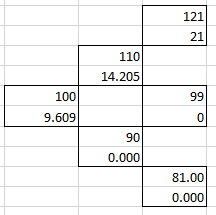
\includegraphics[width=\linewidth]{mod9_p1.png}
\caption{European Call}
\end{subfigure}
\begin{subfigure}{0.4\textwidth}
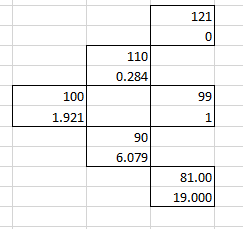
\includegraphics[width=\linewidth]{mod9_p6.png}
\caption{European Put}
\end{subfigure}
\end{figure}
\end{problem}


\begin{problem}{13.11}. $S_0= 40, K = 40, S_0u = 45, S_0d = 35, r = 0.08$. 
\begin{align*}
S_0u \cdot p + S_0d\cdot (1-p) &= S_0\cdot e^{rT} \\
45p + 35(1-p) &= 40 \cdot e^{0.08 \cdot (3/12)} \\ 
p &= 0.5808 \\
f &= e^{-rt}(p\cdot fi_u + (1-p)\cdot f_d) \\
f &= e^{-0.08\cdot (3/12)}(0.5808 \cdot 10 ) \\
f &= 2.847 \\
\hline
45 \Delta - 5 &= 35 \Delta \\
\Delta &= 0.5  && \text{Number of shares to buy per 1 option} \\
45 \cdot 0.5 - 5 &= 17.5 && \text{Value of the portfolio}\\
35 \cdot 0.5 &= 17.5  \\
17.5 \cdot e^{-0.08 \cdot (3/12)} &= 17.15348 && \text{Present value of portfolio} \\
40 \cdot 0.5 - f &= 17.15 && \text{Necessary for no arbitrage} \\
f &= 2.84 && \text{This is the same answer we got before!} 
\end{align*}
\end{problem}

\newpage
\begin{problem}{13.25}. $S_0 = 40, K= 40, r=0.04, \sigma = 0.3, t=(1/4)$. First find u, d, and p for a two step tree. This can be done using the Cox, Ross, Rubinstein parameters for binomial tree (pg. 285,286). We can then use these parameters to construct a binomial lattice tree that can be used to find the value of the option = 3.377 
\begin{align*}
u &= e^{\sigma \cdot \sqrt(t)} &= e^{0.30 \cdot \sqrt(0.25)}  &=  1.162 \\ 
d &= e^{-\sigma \cdot \sqrt(t)} &= e^{-0.30 \cdot \sqrt(0.25)} & = 0.861 \\
a &= e^{rT} &= e^{0.04 \cdot 0.25} &= 1.01 \\
p &= \frac{a-d}{u-d} &= \frac{1.01 - 0.861}{1.162-0.861}  &= 0.49594
\end{align*}

\begin{figure}[h!]
\centering
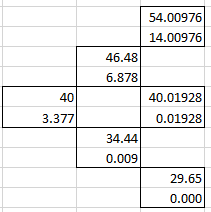
\includegraphics[width=0.5\textwidth]{mod9_p25.png}
\caption{European Call}
\end{figure}
\end{problem}
\end{document}